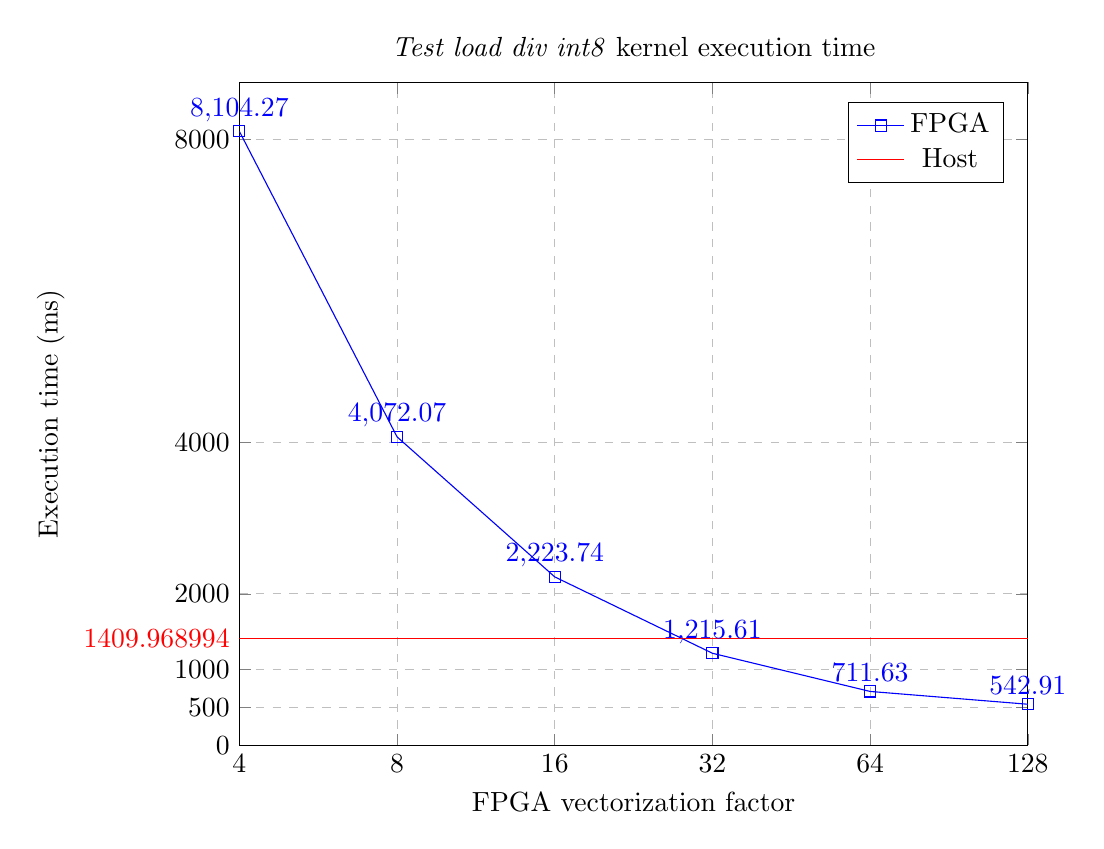
\begin{tikzpicture}
\begin{axis}[
    title={\textit{Test load div int8} kernel execution time},
    xlabel={FPGA vectorization factor},
    ylabel={Execution time (ms)},
    xmin=1, xmax=6,
    ymin=0, ymax=8750,
    xticklabels={4,8,16,32,64,128},
    xtick={1,2,3,4,5,6},
    ytick={0,500,1000,1409.968994,2000,4000,8000},
    yticklabels={0,500,1000,\textcolor{red}{1409.968994},2000,4000,8000},
    legend pos=north east,
    xmajorgrids=true,
    ymajorgrids=true,
    grid style=dashed,
    height=10cm
]
\addplot[color=blue,mark=square, nodes near coords]
    coordinates {
        (1, 8104.273438) (2, 4072.071045) (3, 2223.737061) (4, 1215.6073) (5, 711.628357) (6, 542.909363)
    };
    \addlegendentry{FPGA}

\addplot[color=red]
    coordinates {
        (1, 1409.968994) (2, 1409.968994) (3, 1409.968994) (4, 1409.968994) (5, 1409.968994) (6, 1409.968994)
    };
    \addlegendentry{Host}

\end{axis}
\end{tikzpicture}
